%% Studiendesign.tex
%% $Id: Studiendesign.tex 4 2005-10-10 20:51:21Z bless $
%%

%\chapter{Studiendesign}
%\label{ch:Studiendesign}

%% ==============================
\subsection{Studiendesign}
%% ==============================

\begin{figure}
	\centering
    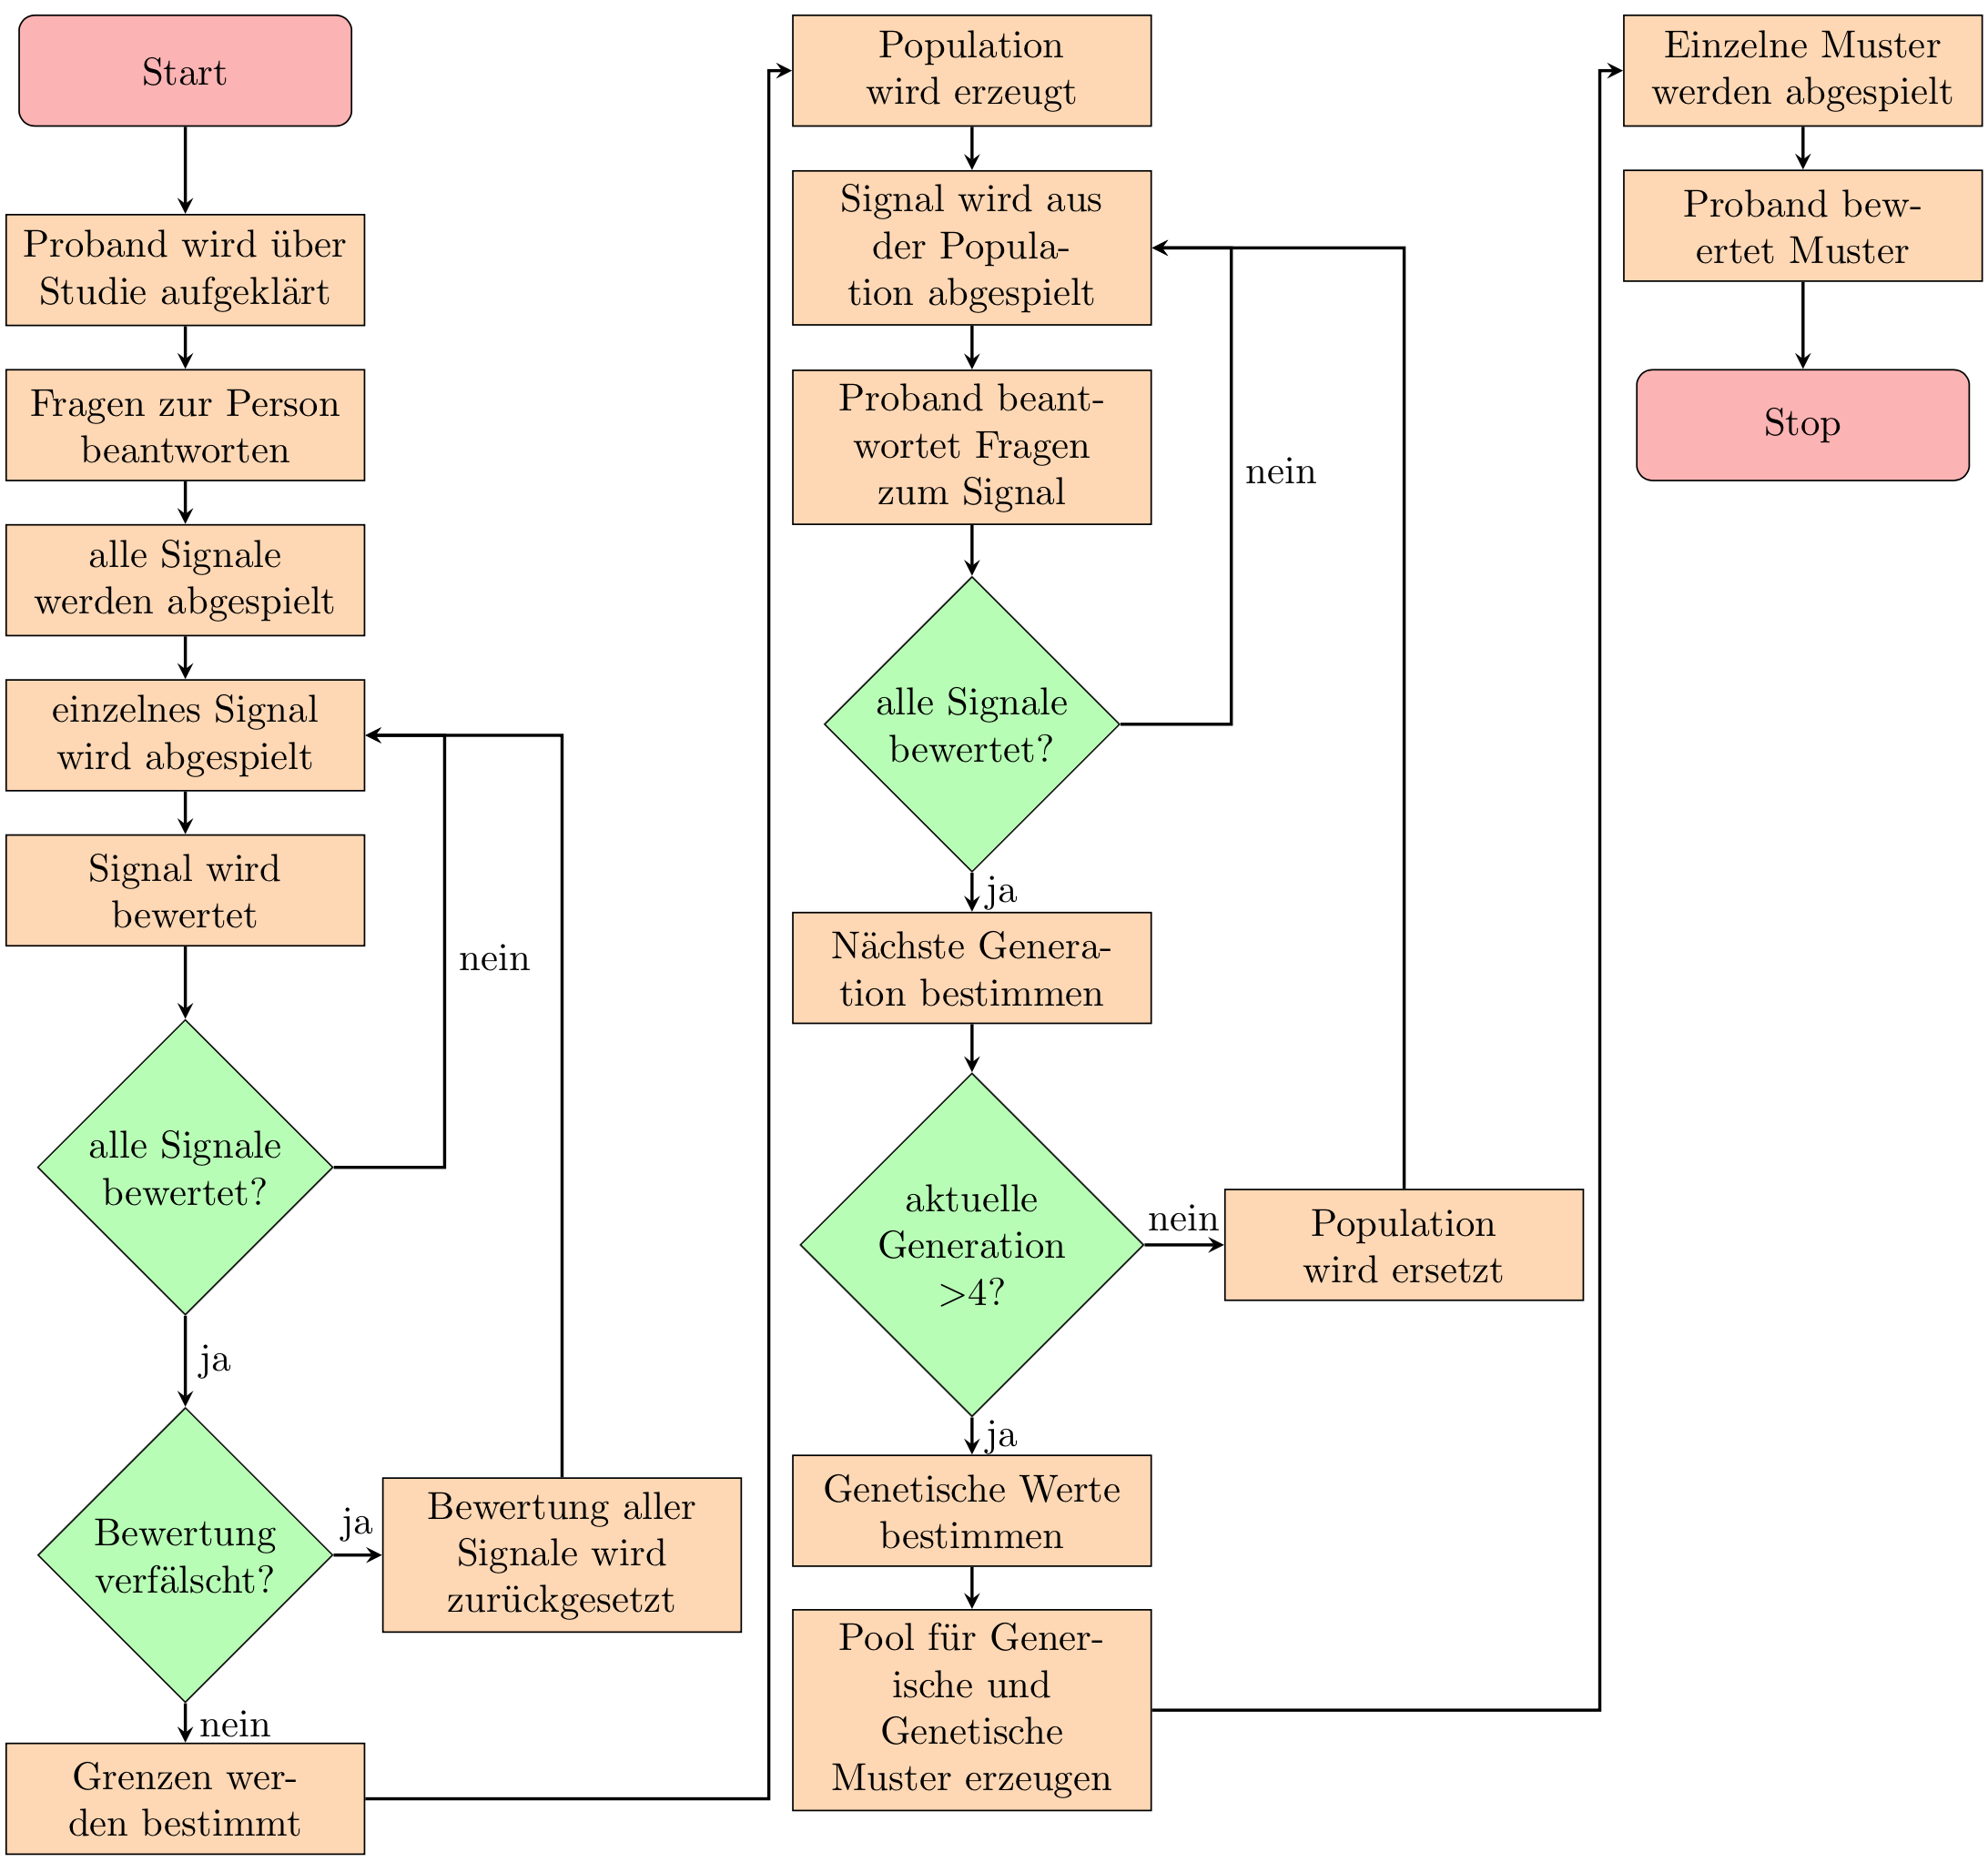
\includegraphics[width=\textwidth]{pics/analyse/Programmablaufdiagramm.png}
    \caption{Studienablauf}
    \label{fig:flussdiagramm}
\end{figure}

Anhand dem folgenden Programmablauf \autoref{fig:flussdiagramm} hat man sich orientiert, um die Studie zu entwerfen. 
{\"U}ber Mailinglisten und Bekanntenkreis haben sich 32 Probanden bereiterkl{\"a}rt an der Studie teilzunehmen. 
Dabei waren 72 Prozent M{\"a}nner und 28 Prozent Frauen. 
Das Alter der Probanden war zwischen 12 bis 54 Jahren vertreten und das Durchschnittsalter war 22 Jahre \autoref{fig:AngabenZurPerson}.  
Die Studie hat zwischen 30 Minuten und einer Stunde gedauert.
Die Studien wurden an drei verschiedenen Orten durchgef{\"u}hrt, im TECO in Karlsruhe, in einem Seminarraum an der Hochschule Darmstadt und in einem Arbeitszimmer in Meschede.

F{\"u}r jeden teilgenommenen Probanden wurde der gleiche Ablauf durchgef{\"u}hrt. 
Vor der Studie wurde ein Termin mit dem Probanden vereinbart. 
Nachdem der Proband zur abgemachten Zeit am vorgegebenen Ort angekommen ist, wurde Ihm erkl{\"a}rt wof{\"u}r die Studie ist, was man mit der Studie herausfinden will und welche Erwartungen man an den Probanden hat. 
Als der Proband alles verstanden hat und die Einverst{\"a}ndniserkl{\"a}rung verstanden und unterschrieben hatte, wurde Ihm das Armband angezogen. Dabei haben die Rechtsh{\"a}nder das Armband an dem linken Arm und die Linksh{\"a}nder an dem rechten Arm angelegt bekommen.

Da man f{\"u}r die Studie ein System mit einer Grafischen Oberfl{\"a}che (GUI) entworfen hatte, wurde der Proband mithilfe des Systems durch die Studie gef{\"u}hrt.
Als nächstes wurden dem Probanden ein paar Personalien abgefragt, wie das Alter, das Geschlecht, ob sich die Person als Musikalisch empfindet, ob man Computerspiele spielen w{\"u}rde, ob man schon einmal eine Smartwatch benutzt habe und ob die Person schon mal ein Tactiles Ger{\"a}t benutzt habe. 
Falls vom Probanden Fragen w{\"a}hrend der Studie Fragen aufgekommen sind wurden diese sofort beantwortet. 

Nach der Aufnahme der Personalien, wurde dem Benutzer erkl{\"a}rt, was Ihn als n{\"a}chstes erwartet und von Ihm verlangt wird. 
Man hat dem Nutzer im ersten Schritt 10 Signale abgespielt, um Ihn ein Gef{\"u}hl f{\"u}r Signale zu geben. 
Im Anschluss wurde dem Probanden jedes Signal einzeln erneut abgespielt. 
Dabei sollte er das Signal zu drei jeweiligen Kategorien zuordnen, die Kategorien waren die Signaltypen \textit{Kurz}, \textit{Mittel} und \textit{Lang}. 
Dieser Schritt war daf{\"u}r notwendig um f{\"u}r den Benutzer die Grenzen f{\"u}r die jeweilige Kategorien zu bestimmen. 
Diese Grenzen sind f{\"u}r die Initialisierung des Algorithmus notwendig gewesen. 

Als die 10 Signale bewertet wurden, wurde der Benutzer dar{\"u}ber aufgekl{\"a}rt, was Ihm als n{\"a}chsten Schritt erwartet. 
Es wurde Ihm ein anhand seiner vorherigen Eingaben eine Population von Signalen erzeugt, es wurde ein zuf{\"a}lliges Signal abgespielt, dass er bewerten sollte.
Mittels drei Fragen wurde das Signal bewertet. 
Um eine Iteration komplett zu bewerten wurde dieser Vorgang 30 mal wiederholt. 
Im Anschluss wurde gefragt wie der Benutzer sich derzeit f{\"u}hlt. 
Nachdem dem der Benutzer eine Iteration komplett bewertet hat, wurden neue Werte berechnet.
%Anhand einer komplett bewerteten Iteration wurde dem Benutzer neue Werte berechnet. 
Es wurden insgesamt vier Iterationen durchgef{\"u}hrt um einen m{\"o}glichst genauen Wert f{\"u}r den Benutzer zu bestimmen.

Im letzten Schritt wurde der Benutzer aufgekl{\"a}rt, dass ab dem Zeitpunkt nur noch Folgen von Signalen, die man ab jetzt Muster nennt, abgespielt werden.
Die Probanden sollten angeben in welcher Reihenfolge was f{\"u}r Signaltypen abgespielt wurden. 
Vor der Studie wurden alle Muster einmalig festgelegt, die jedem Probanden abgespielt wurden.
%Es wurde f{\"u}r alle Probanden im Vorfeld alle Muster definiert, damit jeder die gleichen Muster abgespielt bekommt. 
Es gab zwei Arten von Muster, die generischen Muster und die genetischen Muster. 
Der einzige Unterschied zwischen den beiden Arten waren die Werte, die die Signale in einem Muster zugewiesen wurden. 
Das bedeutet es wurden zwei mal das selbe Muster abgespielt mit lediglich anderen Werten. 
Die Genetischen Muster hatten die Werte, die nach dem Algorithmus erzeugt wurden {\"u}bernommen, wobei die generischen Muster einen vordefinierten Wert zugewiesen bekommen hatten. 
Der generische Wert ist f{\"u}r jeden Probanden gleich gewesen und man hat sich wie im Entwurf schon beschrieben am Paper \cite{pescara2016ruttelflug} orientiert.
Dabei gab es Muster mit drei, vier und f{\"u}nf Signalen. 
Nacheinander wurde dem Nutzer zuerst alle Muster mit drei Signalen, gefolgt von allen Mustern mit vier und zuletzt alle Muster mit f{\"u}nf Signalen abgespielt. 
Das genetische Muster wurde abwechselnd zum generischen Muster abgespielt. 

Nachdem alle Muster von dem Probanden bewertet wurden, haben Sie Ihre e-Mail noch auf Papier angegeben um an einer automatischen Verlosung von zwei Gutscheinen teilzunehmen. 
Bei Interesse wurde Ihnen Ihre Werte gezeigt und erkl{\"a}rt, was genau im Hintergrund passiert worden ist. 
W{\"a}hrend der ganzen Studie standen dem Probanden ausreichend S{\"u}{\ss}igkeiten zur Verf{\"u}gung, bei denen Sie sich frei bedienen konnten.

